\mysubsection{Architecture orientée service (SOA) et ESB}

\ifbook{
  \paragraph{} L'\textbf{Architecture Orientée Services} - ou, en anglais \textit{Service Oriented
  Architecture (SOA)} est probablement l'un des termes les plus à la mode depuis le début des années
  2000. Fruits des années de réflexions sur l'\mylink{}{urbanisation} des systèmes d'informations,
  cette architecture de médiation propose une architecture pour concevoir des systèmes d'information
  très fortement découplé.

  \paragraph{} En effet, l'un des objectifs clairement avoué de cette architecture est de permettre
  la construction de systèmes d'information à l'aide de service hétérogènes, fonctionant sur des
  systèmes et des technologies complètement différentes. On cherche donc ainsi à réaliser des
  logiciels indépendants, exposants différents services métiers ou techniques, chacun
  \textbf{atomique}. Pour réaliser les différents traitements nécessaires à ses utilisateurs, une
  application effectue donc une série d'appel à différents services, et agrège les résultats, avant
  de les présenter à son utilisateur.

  \paragraph{} Néanmoins pour assurer le \textbf{fort découplage} promût par l'architecture, il est
  important qu'une application ne devienne pas adhérante à un service, ce qui reste possible, même
  si ce dernier s'exécute sur une autre machine, dans une autre technologie. L'architecture prévoit
  donc aussi la mise en place de \textbf{contrat de service}, jouant là un rôle similaire à celui
  des \textbf{interfaces} dans le langage de programmation Java. Ces contrats sont placés dans un
  \textbf{annuaire} de service, permettant aux logiciels clients d'accéder de manière transparente
  aux services capables d'assurer les fonctionnalités souhaitées.

  \paragraph{} L'architecture orientée services reste néanmoins très abstraite et n'impose aucune
  technologie pour réaliser les différents éléments nécessaire à son implémentation. Notament, SOA
  ne définit que de manière très lâche les mécanimes à mettre en place pour effectuer la
  communication avec le service, laissant la place à plusieurs protocoles possibles pour
  l'implémenter.

  \mysubsubsection{WebServices}

  \paragraph{} Depuis les débuts de l'informatique, de nombres technologies, standards et
  protocoles\footnote{On ne citera ici que quelques exemples, parmi les plus célèbres: RPC, CORBA,
  COM/DCOM, RPC ...} ont été définies pour permettre de aisément répartir la réalisation de traitements
  entre plusieurs machines distinctes. Nous avons déjà vu par exemple le standard EJB. Au fur et à
  mesure que les systèmes d'information se sont urbanisés, les problématiques d'interopérabilités de
  ces technologies sont apparus de plus en plus clairement, surtout en comparaison avec les progrès
  manifestes réalisés dans le domaine par les technologies internet.

  \paragraph{} S'inspirant donc des idées fortes de ces dernières\footnote{On pense surtout ici au
  côté ouvert du protocole HTTP et de sa communication en format texte (HTML)}, les
  \textit{WebServices} sont donc apparus à leur tour. Utilisant les standards issues de l'émergence
  d'internet - XML, XSD, et définissant son propre ensemble de spécification, dont un format
  d'échange XML nommée \textbf{SOAP}, les \textit{WebServices} ont donc mis tout les chances de
  leurs côtés pour assurer leur interopérabilité.

  \paragraph{} Néanmoins, la complexité des \textit{WebServices} et le foisonement de spécifications
  autour d'elles - ajouté au fait que, malgré les précautions prises, l'interopérabilité fût souvent
  difficile à obtenir, spécialement lorsque les structures de données échangés devinrent de plus en
  plus élaborées, posant encore de des réelles difficultés. Les outils qui devaient résoudre ces
  difficultés ne virent que rarement le jour, et ne tenèrent que rarement leurs promesses.

  \begin{center}
    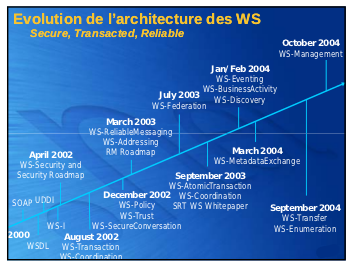
\includegraphics[scale=0.8]{img/ws-star.png}
  \end{center}

  \paragraph{} Un autre aspect, très puissant, des \textit{WebServices} estt la capacité, pour un
  service consommateur de \textbf{négocier} son niveau de protocole. Ceci permettant de gérer les
  problématiques de montée de version d'un service, sans impacter les applications clientes, puisque
  celles-ci devaient être en mesure d'indiquer quel niveau de service - la version du service en
  langage vernaculaire, elle est en mesure d'utiliser.

  \paragraph{} Pour assurer cet aspect et renforcer le découplage entre les consommateurs de
  services et les producteurs, les spécifications \textit{WebServices} prévoient aussi l'utilisation
  d'un annuaire de service, accompagné de sa propre sémantique et norme: UDDI (\textit{Universal
  Description and Discovery Integration}). Ce dernier, dont l'API n'est pas malheureusement la plus
  transparente, a comme fonction de transmettre le point d'accès - ou \textit{endpoint} en anglais,
  soit l'URL a invoquer pour utiliser le service, selon le \textbf{contrat} de service demandé.

  \paragraph{} L'engouement pour les \textit{WebServices} ont rapidement amené à étendre leur
  utilisation. On n'a donc défini des APIs pour standardiser l'utilisation de ces derniers comme
  protocole de communication pour un MOM ou même en tant que canal de communication pour un échange
  RPC ! La nature très verbeuse du protocole ayant souvent un prix en termes de performance, des
  implémentations remplaçant l'utilisation de HTTP et XML par un protocole binaire\footnote{Tel que
  le project Java Hessian} ont vu le jour - même si cette approche peut sembler contre nature...

  \paragraph{} Aujourd'hui, les \textit{WebServices} disposent donc d'un écosystème riche et fourni,
  mais l'enthousiasme les concernants à largement réduit, suite aux difficultés rencontrées sur le
  terrain, lors de leurs implémentations. Si ils se révèlent une technologie robuste et
  intéropérable pour mettre en place des services métiers complexes - et souvent orientés "écriture
  de données", ils se sont souvent révélés inadapté à des cas d'utilisation plus simple, et aussi
  souvent orienté "lecture" de données.

  \paragraph{} Le fait que Google a retiré depuis maintenant plusieurs années son API SOAP
  \footnote{au profit d'un nouveau type d'API que nous allons maintenant évoquée} est un indicateur
  fort du recul des \textit{WebServices} comme solution "parfaite" pour la conception de services
  distants ou internet.

  \paragraph{} \paragraph{} \textit{Remarque: Si la notion d'architecture orienté service n'impose
  en aucun cas l'utilisation de WebService\footnote{Pour s'en convaincre, il suffira d'étudier la
  page Wikipedia associée à
  \mylink{http://en.wikipedia.org/wiki/Service_Oriented_Architecture_Fundamentals}{SOA}}, ces
  derniers adressent la plupart des contraintes et recommandations de SOA. Il faut néanmoins noter
  que des projets respectant les principes de SOA ont  été implémenté, avec succès, à l'aide
  d'autres technologie telle RMI ou ReST. Il est donc important de retenir que SOA n'implique pas
  obligatoirement l'utilisation de \textit{WebServices}}.
}


\ifslide{
  \begin{frame}{Web Service}
    \begin{block}{Qu'est qu'un \textit{Web Service}}
      \begin{itemize}
        \item même concept que le Web mais appliqué la communication entre machine
        \item donc moins orienté "lecture" (plus d'opération d'écriture)
        \item plus "dynamic"
        \item support des environements hétérogènes
      \end{itemize}
    \end{block}
  \end{frame}

  \begin{frame}{Web Service}
    \begin{block}{Indépendance du \textit{End Point}}
      \begin{itemize}
        \item traitement réparti
        \item maintenance du noeud indépendante
        \item négociation de protocole
        \item couplage lâche
      \end{itemize}
    \end{block}
  \end{frame}

  \begin{frame}{Web Service}
    \begin{block}{Composition de protocole}
      \begin{itemize}
        \item architecture modulaire
        \item complexité géré par les outils
        \item extensibilité apporté par XML
      \end{itemize}
    \end{block}

    \begin{center}
      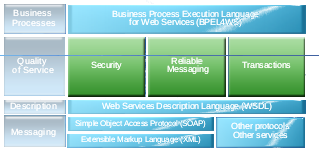
\includegraphics[scale=0.8]{img/web-services.png}
    \end{center}

  \end{frame}

  \begin{frame}{Web Service}
    \begin{center}
      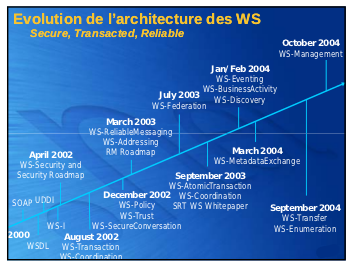
\includegraphics[scale=0.8]{img/ws-star.png}
    \end{center}
  \end{frame}

  \begin{frame}
    \begin{block}{MOM et RPC... en WS !}
      \begin{itemize}
        \item XML-RPC
        \item publish/subscribe
        \item pièce jointe
      \end{itemize}
    \end{block}

    \begin{block}{Indépendance du transport}
      \begin{itemize}
        \item HTTP
        \item TCP
        \item Binaire !
      \end{itemize}
    \end{block}
  \end{frame}

  \begin{frame}
    \begin{block}{Mais aussi...}
      \begin{itemize}
        \item transaction
        \item sécurité
        \item ...
      \end{itemize}
    \end{block}

    \begin{block}{Découverte de Service et Annuaire}
      \begin{itemize}
        \item UDDI
        \item WS-Discovery
      \end{itemize}
    \end{block}
  \end{frame}
}

\ifbook{
  \mysubsubsection{ReST - le successeur des WebServices ?}

  \paragraph{} Si les \textit{WebServices} sont clairement issus du monde de l'industrie et le fruit
  d'un travail de standardisation, ReST n'est pas un standard, ni même une technologie réellement
  définie. ReST - ou \textit{Representationnal State Transfer} en anglais, est en quelque sorte le
  fruit d'un analyse des bonnes pratiques, en terme d'architecture, qui ont émergés sur l'ensemble
  de l'internet.

  \paragraph{} Sans rentrer dans les détails de sa théorie\footnote{On pourra là aussi consulter la
  page wikipédia consacré à \mylink{TODO}{ReST}.}, nous pourrons retenir que ReST tant à simplifier
  la communication entre le client et le serveur en exploitant autant que possible les mécanismes
  offerts par le protocole HTTP (utilisation de l'ensemble des opérations du protocole, soit PUT et
  DELETE, et non seulement des méthodes POST, mais aussi utilisation d'une sémantique très
  expressives dans les URLs des services), plutôt que de transmettre de descripteurs multiples en
  XML, par exemple.

  \paragraph{} Sur le format de données, ReST n'impose rien, mais, de plus en plus, l'usage impose
  l'utilisation du format JSON, issu du monde Javascript, et considéré par une partie de
  l'industrie, comme beaucoup plus clair et approprié que XML. Néanmoins, si les services de types ReST
  ont d'indéniables avantages, il est peut être un peu hasardeux de les positionner comme une
  technologie de remplacement des \textit{WebServices}.

  \paragraph{} En effet, si il est appararu clairement que ces derniers n'étaient pas adapté à la
  mise en place de service de consultation donnée à grande échelle (sur internet), les services de
  types ReST posent de grandes difficultés dans la réalisation de services applicatifs - ces
  derniers ne proposent que peu de solutions pratiques ou standard dans le domaine de la sécurité,
  ou de la transaction, par exemple.

  \paragraph{} En guise de conclusion de très haut niveau, on pourra donc retenir que les services
  de types ReST sont généralement très adaptés à la mise en place de services en "lecture", devant
  fournir un accès des données pour de buts de consultations. À l'inverse, les \textit{WebServices}
  se révèlent un ensemble de standards assez complet pour la conception de services nécessitant
  la modification ou l'ajout de données.\footnote{Il s'agit bien évidemment d'une conclusion très
  générale, pour éclairer le lecteur sur ces technologies, et non de la définition d'une règle
  absolu et unilatéral. Face au choix Rest ou \textit{WebServices}, le lecteur devra prendre soin
  d'analyser en détail les cas d'utilisations et le contexte techniques avant d'opter pour l'une ou
  l'autre des technologies.}
}


\ifbook{
  \mysubsubsection{SOA et Bus logiciel (ESB)}

  \paragraph{} Faisons un rapide bilans des nombreuses technologies évoqués dans ce chapitre et les
  précédents de cette ouvrage. On se rend compte ainsi que le système d'informations, désormais très
  urbanisé, contient beaucoup d'élément hétérogènes:

  \begin{itemize}
    \item \textit{WebServices} et service ReST,
    \item MOM,
    \item BPM et leur moteur de règles,
    \item ...
  \end{itemize}

  \paragraph{} Il apparait évident qu'une application métier pour réaliser ses fonctionnalités va
  devoir faire appel à ses différents éléments et que très rapidement un besoin
  d'\textbf{orchestration} de ces différents services va apparaitre. En effet, dans une vision
  \textbf{opérationnel} du système d'information, il apparait important, si ce n'est essentiel, de
  disposer, entre les consommateurs de services et leurs fournisseurs d'un mécanisme pour effectuer
  de la \textbf{répartition de charge} ou du simple \textbf{routage}, comme par exemple lors de
  l'interromption, pour maintenance ou mise à une jour, d'une instance d'un service.

  \paragraph{} C'est de ce besoin qu'a émergé la notion de \textit{Entreprise Service Bus (ESB)}. En
  effectuant un parallèle avec les bus de communication électroniques, ces solutions se positionnent
  donc comme un intermédiaire similaire, et pourtant presque invisible, entre les consommateurs et
  fournisseurs de services.

  \paragraph{} En outre, ces outils permettent aussi d'effectuer des \textbf{transformation} de
  données ou de protocole, pour permettre à deux services - à priori incompatibles, de communiquer
  malgré tout. À ce regard, les ESB sont les hérities des EAI - \textit{Entreprise Application
  Integration}, qui effectue le même genre de synthèse, mais sur des technologies et protocoles
  non standard issus des logiciels propriétaires.\footnote{Là encore, le lecteur prendra soin de
  noter que cette synthèse est relativement grossière et quelques peu simpliste.}

  \begin{center}
    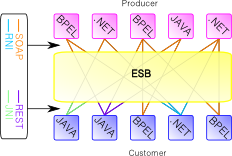
\includegraphics[scale=1]{img/esb.png}
  \end{center}

  \paragraph{} \textit{\mylink{http://en.wikipedia.org/wiki/BPEL}{BPEL}: Business Process Execution
  Language est un langage de programmation destiné à l'exécution des procédures d'entreprise.}
}

\ifslide{

  \begin{frame}
    \begin{block}{SOA}
      \begin{itemize}
        \item architecure
        \item \textit{loose coupling}
        \item fonctionnement par contrat
      \end{itemize}
    \end{block}

    \begin{block}{ESB}
      \begin{itemize}
        \item orchestration
        \item analogue à un Bus électronique
      \end{itemize}
    \end{block}
  \end{frame}

  \begin{frame}{ESB}
    \begin{center}
      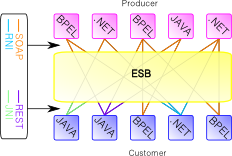
\includegraphics[scale=1]{img/esb.png}
    \end{center}
  \end{frame}

}
